
\subsection{Perancangan \textit{Database}}
Pada subbab ini akan dijelaskan bagaimana rancangan basis data yang digunakan pada aplikasi lelang \textit{online} ini. Sistem basis data yang digunakan pada aplikasi ini menggunakan dua jenis database, yaitu transaksional (menggunakan PostgreSQL) dan nontransaksional (menggunakan MongoDB). \textit{Conceptual Data Model} (CDM) dan \textit{Physical Data Model }(PDM) dari basis data sistem ini dijelaskan pada Gambar \ref{cdm} dan Gambar \ref{pdm}.
	\subsubsection{\textit{Conceptual Database Model}}
	\begin{figure}[H]
		\centering
		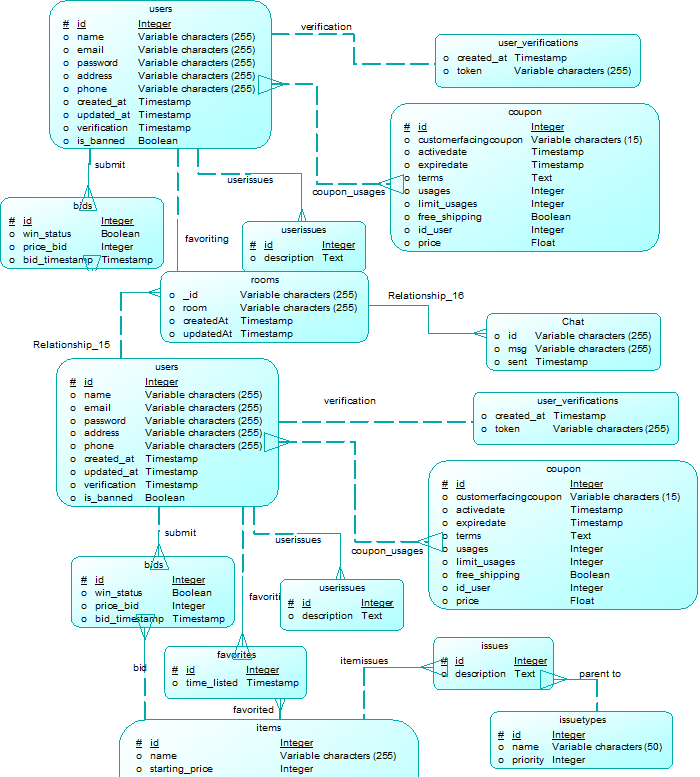
\includegraphics[width=\textwidth]{images/bab3/db/cdm.png}
		\caption{\textit{Conceptual Database Model} (PDM) Aplikasi}
		\label{cdm}
	\end{figure}
	
	
	\subsubsection{\textit{Physical Database Model}}
	\begin{figure}[H]
		\centering
		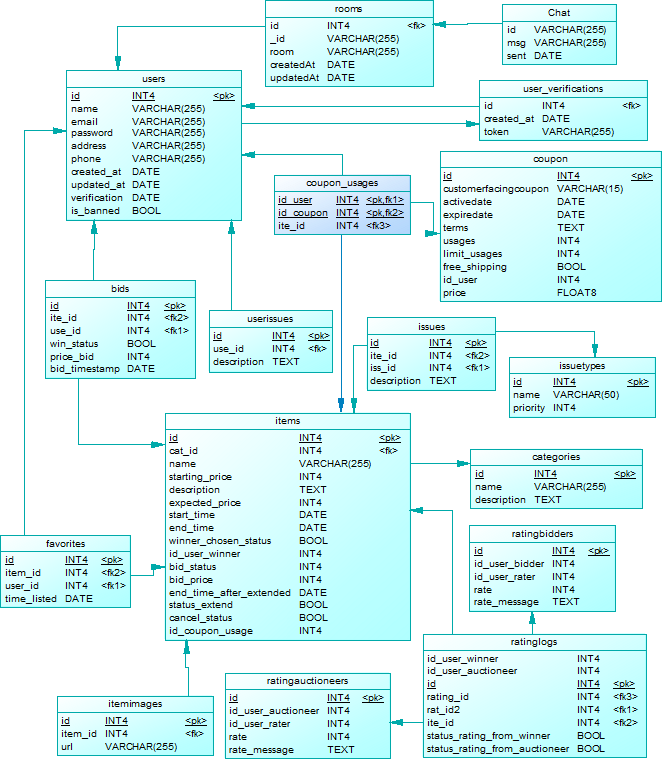
\includegraphics[width=\textwidth]{images/bab3/db/pdm.png}
		\caption{\textit{Physical Database Model} (PDM) Aplikasi}
		\label{pdm}
	\end{figure}
	
%  Konsep Item Caching
%  Pyshical Database Design
%   	 \begin{longtable}{|r|X|X|X|}
 	\caption{Kamus Data Tabel \textit{users}}
 	\label{db-users} \\ \hline
 	\textbf{No} & \textbf{Nama Atribut} & \textbf{Tipe Data} & \textbf{Keterangan} \\ \hline
 	\endfirsthead
 	
 	\multicolumn{4}{c}%
 	{\tablename\ \thetable{} -- lanjutan dari halaman sebelumnya} \\ \hline
 	\textbf{No} & \textbf{Nama Atribut} & \textbf{Tipe Data} & \textbf{Keterangan} \\ \hline
 	\endhead
 	
 	\hline
 	\endlastfoot
\multicolumn{1}{|c|}{	1	}&	id	&	int	&	PK, Autoincrement	\\ \hline
\multicolumn{1}{|c|}{	2	}&	name	&	varchar(255)	&	Nama	\\ \hline
\multicolumn{1}{|c|}{	3	}&	email	&	varchar(50)	&	Email	\\ \hline
\multicolumn{1}{|c|}{	4	}&	password	&	varchar(255)	&	Password	\\ \hline
\multicolumn{1}{|c|}{	5	}&	address	&	text	&	Alamat	\\ \hline
\multicolumn{1}{|c|}{	6	}&	phone	&	varchar(50)	&	No. HP	\\ \hline
\multicolumn{1}{|c|}{	7	}&	created\_at	&	timestamp	&	Timestamp	\\ \hline
\multicolumn{1}{|c|}{	8	}&	updated\_at	&	timestamp	&	timestamp	\\ \hline
\multicolumn{1}{|c|}{	9	}&	username	&	varchar(20)	&	Username	\\ \hline
\multicolumn{1}{|c|}{	10	}&	verification	&	timestamp	&	Tanggal user terverifikasi - jika belum diverifikasi, isinya NULL	\\ \hline
\multicolumn{1}{|c|}{	11	}&	is\_banned	&	timestamp	&	Status banned pengguna	\\ \hline

 \end{longtable}
    